\documentclass[11pt]{article}
\usepackage{fullpage,amsthm,amsfonts,amssymb,epsfig,amsmath,times,amsthm,listings,color, graphicx}

\definecolor{dkgreen}{rgb}{0,0.6,0}
\definecolor{gray}{rgb}{0.5,0.5,0.5}
\definecolor{mauve}{rgb}{0.58,0,0.82}

\lstset{frame=tb,
  language=Java,
  aboveskip=3mm,
  belowskip=3mm,
  showstringspaces=false,
  columns=flexible,
  basicstyle={\small\ttfamily},
  numbers=none,
  numberstyle=\tiny\color{gray},
  keywordstyle=\color{blue},
  commentstyle=\color{dkgreen},
  stringstyle=\color{mauve},
  breaklines=true,
  breakatwhitespace=true,
  tabsize=3
}

\newtheorem{theorem}{Theorem}
\newtheorem{claim}[theorem]{Claim}

\begin{document}

\begin{text} 
Davie Truong\\
“I have read and agree to the collaboration policy. Davie Truong”\\
Homework Heavy \\
\end{text}


\begin{center}
{\bf\Large CMPS 102 --- Spring 2017 --  Homework 2}
\end{center}

\section*{Solution to Problem 3}

\begin{text} 
a)
This algorithm does not always find the smallest set of nurses because by choosing the nurse with the longest time, it ignores the nurse with a short interval, but covers more effectively. More specifically, the longest time can cover the open shift for a short amount, but for the rest of the shift, the nurse is overlapping with another nurse. Where as a nurse with a shorter time can cover the open shift for a longer period while not having longer time for overlapping with the previous nurse. 
\begin{figure}[h]
\centering
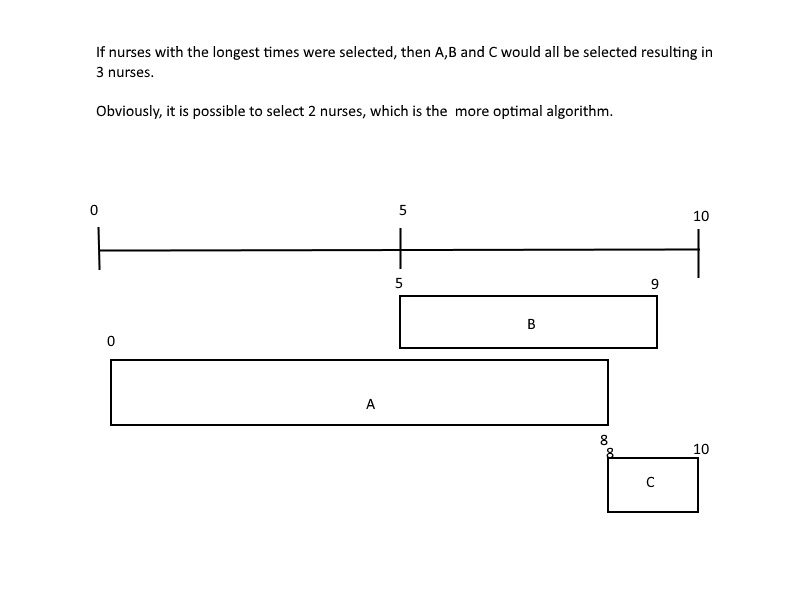
\includegraphics[width=100mm]{nurseGraphic}
\end{figure}
\end{text}

\section*{Algorithm} 
b)
-consider shifts in increasing order of start time  \\
-want to choose by finish time that is highest while maintaining a start that is compatible\\
-remember nurse i* that was added last to A \\
-nurse i is compatible with A if $S_i* <= S_i <= F_i*$ or for the start where $S_i$ must equal 0 to be compatible \\
\begin{lstlisting}
A <- null 	// A is empty array to store nurse shifts
while ( i has not gone through all shifts i.e. reach n)
	if ( i is compatible)
		temp is assigned i
		x = i + 1	// the next value on the sorted list
		while ( A has not been assigned a shift)
			if ( x is not compatible with As current shift)
				A <- temp
				i = x 		// so the main loop isn't redundant 
			else 		// x is compatible, this is to find greatest compatibility with greatest finish time
				temp = x 
				x =- x + 1 	// the next value on the list
				if ( temp is equal to n)
					A <- temp
					i = x 		// not really necessary since the return will exit the loop
					return A
	else 	// if i is not compatible 
		return  "no such subset exist"
\end{lstlisting}

\begin{text} 
Description:
The algorithm works by using the start time as the order to iterate through the list. It then checks each following shift in the list for highest finish time while maintaining compatibility. The shift that fits the requirement gets added to the "schedule" If the shift is not compatible that means there is a gap in the schedule leaving no nurse to tend Mr. Banks. 
\end{text}

\begin{proof}
\begin{text}
c) Proof of Correctness:\\
The algorithm will terminate: The algorithm runs until all nurses have been considered (i = n). The inner while loop updates this i every time it checks for compatibility and tries to find a nurse with a higher finish time. Therefore the algorithm will end with a completed schedule or no schedule if there is a gap in the availability of nurses.\\
Greedy Algorithm is optimal: \\
Proof by contradiction:\\
-Assume greedy is not optimal\\
-Let $i_1, i_2,..., i_k$ denote the shifts selected by greedy\\
-Let $j_1,j_2,..., j_k$ denote the shifts in the optimal solution \\
-With $i_1  = j_1, i_2 = j_2, ..., i_r = j _r$ for the largest possible value of r. \\
-The shift $j_r+1$ chooses shifts that must be compatible by definition of the algorithm.\\
-The shift $j_r+1$ can't choose shifts with low finish times because that would cause overlapping and a greater number of nurses to be hired, there fore it must choose shifts with highest finish times. However, this is the greedy algorithm therefore, $i_r+1 >= j_r+1$  by greedy choice of the algorithm.
\end{text}
\end{proof}

\section*{Analysis}

\begin{text}
Time Complexity: \\
$O(n^2)$ \\
-n to sort the algorithm and n again to consider all the nurse's shifts and their compatibility with the schedule while maintaining the lowest amount of nurses picked
\end{text}

\begin{text}
Space Complexity: \\
O(n)\\
-worse case it takes all nurses if shifts are side by side\\
-since we are working on the 1 array and not needing any other space
\end{text}

\end{document}
